\section{Experimental Protocol}
\label{sec:protocol}
\subsection{Chronology and selection}
The initial development history is 2010--2018, validation uses holding intervals within 2019--2021, and final testing uses holding intervals within 2022--2025. An interval belongs to a reporting period only if its entry is on or after the period start and its exit is on or before the period end. The first holdout signal is therefore formed at the 31 December 2021 close, for entry on 3 January 2022. The final exit is the 31 December 2025 open. No 2021 holding return enters the test merely because its signal date precedes entry.

\begin{figure*}[t]
 \centering
 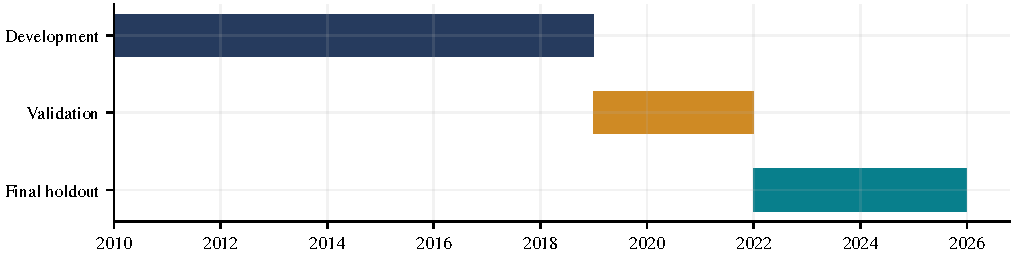
\includegraphics[width=\textwidth]{generated/timeline.pdf}
 \caption{Frozen chronology. Each monthly fit uses only the latest 1,260 outcomes that have matured at the decision close. Validation selects the penalty; the final holdout evaluates only that selection. The split refers to executable holding intervals, not merely feature timestamps.}
 \label{fig:timeline}
\end{figure*}

Each of the four candidates is walked forward through the validation period, with scaling and model parameters fitted only on past eligible observations. The candidate with the highest net validation Sharpe at 5 bps is selected; ties within $10^{-12}$ choose the larger $\alpha$. Table~\ref{tab:validation} gives the complete declared grid. Penalties 0.1 and 1 produce the same validation position path, although their continuous forecasts differ. The tie rule selects $\alpha=1$.

\begin{table}[t]
 \centering\small
 \caption{Validation-only selection, 2019--2021. All returns include 5 bps single-side costs.}
 \label{tab:validation}
 \resizebox{\columnwidth}{!}{\begin{tabular}{lrrr}
\toprule
$\alpha$ & CAGR (\%) & Net Sharpe & Exposure (\%) \\
\midrule
0.1 & 22.33 & 1.2060 & 76.72 \\
1 & 22.33 & 1.2060 & 76.72 \\
10 & 19.15 & 1.0767 & 77.38 \\
100 & 18.64 & 1.0310 & 85.71 \\
\bottomrule
\end{tabular}
}
\end{table}

The selection artifact stores the protocol digest, raw-data digest, validation-table digest, candidate count, and selected penalty. The final-test routine checks those fingerprints and fits only the selected penalty. Repeating the identical pipeline verifies reproducibility; it does not provide a fresh independent holdout. No feature, threshold, window, or model-family change is justified using these test results.

The holdout contains \OutcomeCount{} return intervals and \FitCount{} model fits: an initial fit on the last session of 2021 and scheduled fits at the first decision session of each month in 2022--2025. Earlier holdout outcomes can enter later rolling windows after they mature. That scheduled updating differs from reselecting a strategy after observing its test performance.

The design was fixed before the first market-data download in this implementation on 9 November 2026. It is not an externally preregistered prospective test: these market years were already historical, and researchers may know their broad behavior. The artifact lock documents the implemented sequence, not a stronger guarantee about historical research independence.

\subsection{Evaluation measures}
For net interval returns $R_i=G_i-1$, with final liquidation included, define
\begin{align}
 \mathrm{CAGR} &= V_N^{252/N}-1,\label{eq:cagr}\\
 \widehat\sigma_{\mathrm{ann}} &= \sqrt{252}\,
 \operatorname{sd}_{N-1}(R_1,\ldots,R_N),\\
 \widehat{\mathrm{SR}} &=
 \frac{252\,\overline R}{\widehat\sigma_{\mathrm{ann}}}.
 \label{eq:sharpe}
\end{align}
The Sharpe reference rate is zero, consistent with the cash assumption. It is not an estimate of excess performance over realized Treasury returns. Arithmetic annualized return is $252\overline R$, reported separately from CAGR. Maximum drawdown is the minimum wealth-to-running-peak ratio minus one, with initial wealth one included in the peak. Turnover counts both initial entry and terminal liquidation.

Forecast error is assessed against a historical-mean forecast $\bar y_{d(t)}$ estimated from the same mature training sample at each refit:
\begin{equation}
 R^2_{\mathrm{OOS}}=1-
 \frac{\sum_i(y_i-\widehat y_i)^2}
 {\sum_i(y_i-\bar y_{d(i)})^2}.
 \label{eq:r2}
\end{equation}
This is neither in-sample explained variance nor a comparison with the holdout mean. Annual return tables use the continuous net portfolio path, without artificial December liquidation and January repurchase.

\begin{algorithm}[t]
 \caption{Time-respecting selection and evaluation}
 \label{alg:rolling}
 \begin{algorithmic}[1]
  \Require Trailing features, labeled exit dates, fixed grid $\mathcal A$
  \For{$\alpha\in\mathcal A$}
   \For{validation decision close $t$, in order}
    \If{first signal or new decision month}
     \State Select $\mathcal T_t$ by Eq.~\eqref{eq:eligible}
     \State Fit scaler and Ridge on $\mathcal T_t$
    \EndIf
    \State Forecast and set $w_t$ by Eq.~\eqref{eq:position}
   \EndFor
   \State Account for costs, entry, and liquidation
  \EndFor
  \State Select $\alpha^*$ by validation net Sharpe
  \State Lock protocol, data, and selection digests
  \State Walk forward on holdout using $\alpha^*$ only
  \State Save forecasts, fit audits, wealth, and metrics
 \end{algorithmic}
\end{algorithm}

\section{Results}
\label{sec:results}
\subsection{Net performance does not beat the passive alternative}
Table~\ref{tab:headline} reports the full-period holdout results at 5 bps. Ridge earns \RidgeCAGR{} CAGR and a \RidgeSharpe{} Sharpe, compared with \BHCAGR{} and \BHSharpe{} for buy-and-hold. Its total net return is 28.63\%, versus 52.38\% for the passive alternative. It exceeds the fixed moving-average rule on CAGR and Sharpe, but outperforming another timing rule is insufficient to establish economic value when an investable passive benchmark does better.

\begin{table*}[t]
 \centering\small
 \caption{Final holdout, 2022--2025: net performance at 5 bps single-side cost. All strategies share entry and exit dates, dividend treatment, and cost conventions. Returns and volatility are annualized with 252 intervals; total return and exposure are not annualized.}
 \label{tab:headline}
 \begin{tabular}{lrrr}
\toprule
Metric & Ridge & MA20 & Buy-and-hold \\
\midrule
CAGR (\%) & 6.54 & 3.69 & 11.18 \\
Arithmetic return (\%) & 7.56 & 4.22 & 12.27 \\
Volatility (\%) & 15.72 & 10.83 & 18.31 \\
Sharpe ($r_f=0$) & 0.481 & 0.389 & 0.670 \\
Max. drawdown (\%) & -22.20 & -19.14 & -26.28 \\
Total return (\%) & 28.63 & 15.52 & 52.38 \\
Equity exposure (\%) & 69.36 & 65.27 & 100.00 \\
One-way turnover & 246 & 102 & 2 \\
\bottomrule
\end{tabular}

\end{table*}

\begin{figure*}[t]
 \centering
 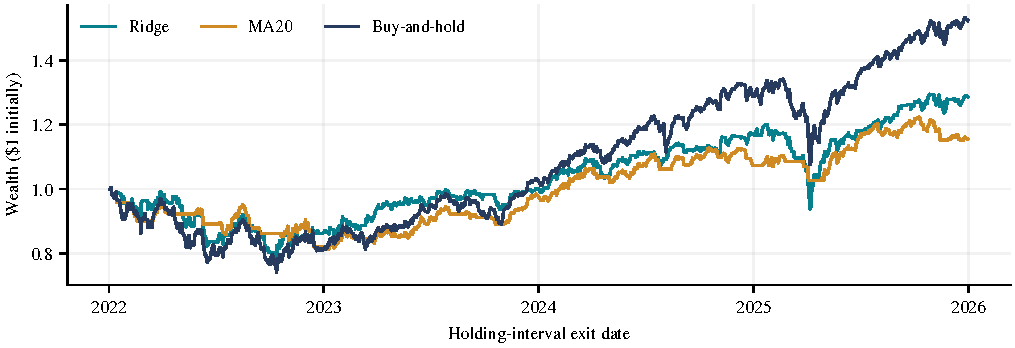
\includegraphics[width=\textwidth]{generated/wealth.pdf}
 \caption{Cumulative net wealth. Every strategy begins with one unit of capital and pays entry and terminal-liquidation fees. Ridge's reduced participation limits losses in some intervals but also sacrifices gains. The plotted trajectory is the frozen holdout path, not a selected subperiod.}
 \label{fig:wealth}
\end{figure*}

Figure~\ref{fig:wealth} shows the cumulative paths. Final wealth is approximately 1.286 for Ridge, 1.155 for MA20, and 1.524 for buy-and-hold. A strategy that spends time in cash must avoid enough adverse returns to compensate for forgone positive exposure and extra fees. The positive average return of the underlying during the holdout makes this hurdle economically relevant. The figure also discourages extrapolating from the strategy's stronger validation period or a single favorable test year.

\subsection{Costs erase approximate gross Sharpe parity}
The zero-cost Ridge Sharpe is 0.678, compared with 0.672 for buy-and-hold. This approximate numerical parity should not be interpreted as a statistically significant difference. It disappears at the main implementation cost: Ridge's net Sharpe is 0.481, while the benchmark changes little because it trades only twice. Figure~\ref{fig:cost} varies fees on the same fixed positions. At 10 bps, Ridge's CAGR is 3.29\% and Sharpe is 0.284; no new model is selected for any cost scenario.

\begin{figure}[t]
 \centering
 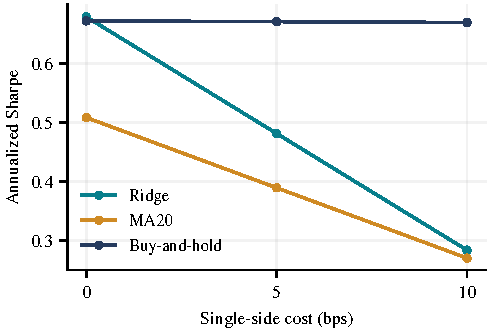
\includegraphics[width=\columnwidth]{generated/cost_sharpe.pdf}
 \caption{Cost sensitivity of fixed positions. Ridge generates 246 charged one-way trade units, MA20 102, and buy-and-hold 2. The cost scenarios reprice the same experiment.}
 \label{fig:cost}
\end{figure}

The mechanism is quantitatively specific. Ridge's annualized turnover is approximately 61.87 units, versus 0.50 for buy-and-hold over this finite entry-to-liquidation sample. From Proposition~\ref{prop:drag}, its net-to-gross terminal wealth ratio is $(1-0.0005)^{246}\approx0.8842$. This is approximately 3.09\% annual log-wealth drag. The corresponding benchmark ratio is $(1-0.0005)^2\approx0.9990$. Cost sensitivity is therefore linked to a verifiable accounting identity, rather than inferred only from a visual change in the Sharpe curve.

This result does not establish that 5 bps is a universal estimate of SPY opening-auction execution costs. It is a fixed research assumption, with zero and 10 bps included to expose sensitivity. Nor does it imply that a cost-aware threshold would fail. Such a threshold is a different strategy requiring its own selection and evaluation; it is not retrofitted here.

\subsection{Risk reduction is accompanied by lower exposure}
Ridge's annualized volatility is 15.72\%, below the benchmark's 18.31\%. Maximum drawdown improves from \BHMDD{} to \RidgeMDD{}. Figure~\ref{fig:drawdown} shows that the strategy still suffers substantial peak-to-trough losses. MA20 reduces volatility further, to 10.83\%, but also earns the lowest CAGR. These comparisons demonstrate a risk--growth trade-off rather than a uniform ordering of strategies.

\begin{figure*}[t]
 \centering
 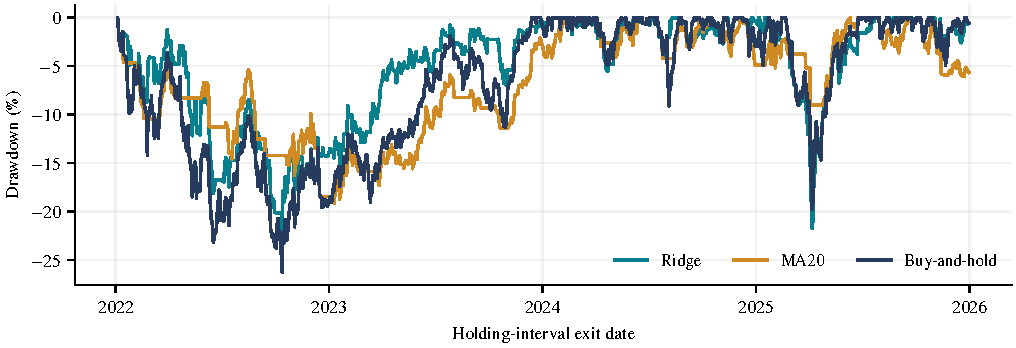
\includegraphics[width=\textwidth]{generated/drawdown.pdf}
 \caption{Net drawdowns, including initial wealth in the running peak. Lower drawdown is considered jointly with growth, Sharpe, and equity exposure. It is not a bound on future losses or evidence of successful crash prediction.}
 \label{fig:drawdown}
\end{figure*}

Average Ridge exposure is \RidgeExposure{}. A constant fractional exposure equal to that realized test average gives an ex post, gross diagnostic with 8.03\% CAGR, 12.70\% volatility, and 0.672 Sharpe. It uses holdout information and excludes fractional rebalancing costs; it is therefore not an investable comparator. Its role is limited: it illustrates why holding less equity can reduce volatility without establishing selection skill. A genuine risk-matched benchmark would need a pre-test exposure choice or a pre-specified adaptive rule.

\subsection{Prediction accuracy supplies no independent rescue}
The model's $R^2_{\mathrm{OOS}}$ is \OOSRsquared{} against the past-only historical mean. Model MSE is 0.00013365, versus 0.00013293 for the baseline. Thus the model does not improve squared-error prediction in the final period. Directional accuracy is \HitRate{}, a descriptive statistic that ignores the unconditional fraction of positive intervals, return magnitudes, and costs.

The sign-based portfolio rule is especially sensitive to the distinction between prediction and action. Magnitude information is discarded after zero-thresholding: a tiny positive forecast produces the same full position as a larger forecast. Small changes around zero can cause a full turnover event. Forecast scatter, the distribution of scores, a confusion matrix, and realized returns conditional on the frozen decisions appear in Appendix~\ref{app:empirical}. Those tables diagnose the same path; they are not used to select another threshold.

\subsection{The full-period finding is not a single-year effect}
\begin{table}[t]
 \centering\small
 \caption{Calendar-year compounded net returns. The portfolio path is continuous across year boundaries.}
 \label{tab:annual}
 \resizebox{\columnwidth}{!}{\begin{tabular}{lrrr}
\toprule
Year & Ridge (\%) & MA20 (\%) & Buy-and-hold (\%) \\
\midrule
2022 & -13.80 & -17.99 & -18.82 \\
2023 & 16.15 & 19.93 & 27.09 \\
2024 & 16.90 & 9.09 & 25.40 \\
2025 & 9.88 & 7.67 & 17.79 \\
\bottomrule
\end{tabular}
}
\end{table}
Ridge loses less than buy-and-hold in 2022, but trails it in 2023, 2024, and 2025 (Table~\ref{tab:annual}). The improvement in one down-market year is not sufficient to offset lower growth in subsequent years. Annual Sharpe estimates are short-sample descriptions, not reliable long-run parameters. We do not switch strategies retrospectively between calendar years or claim that observed annual differences establish a stable market regime rule.

The coefficient paths are also descriptive. Rolling estimates can change as old outcomes leave the fixed window and new outcomes become available. Changes may reflect a shifting relation, correlated predictors, or estimation noise. They do not authorize removing a feature after seeing the test period. Full monthly fit boundaries and coefficient summaries are retained in the supplement so that this limitation is visible rather than hidden behind the aggregate result.
